\documentclass{article}
\usepackage[utf8]{inputenc}
\usepackage[german]{babel}
\usepackage{graphicx} 
\usepackage{amsmath}

\usepackage[square,numbers]{natbib}
\bibliographystyle{abbrvnat}

\title{Aufbau und Justage eines Leckstrahlmikroskopes zum Nachweis des plasmonischen Spin-Hall-Effektes}
\author{Hanno Christiansen}
\date{März 2021}

\begin{document}
	
\maketitle
\tableofcontents

\section{Einführung}
\section{Theorie}
	\subsection{Oberflächen-Plasmon-Polariton (SPP)}
	\begin{figure}[htbp] 
		\centering
		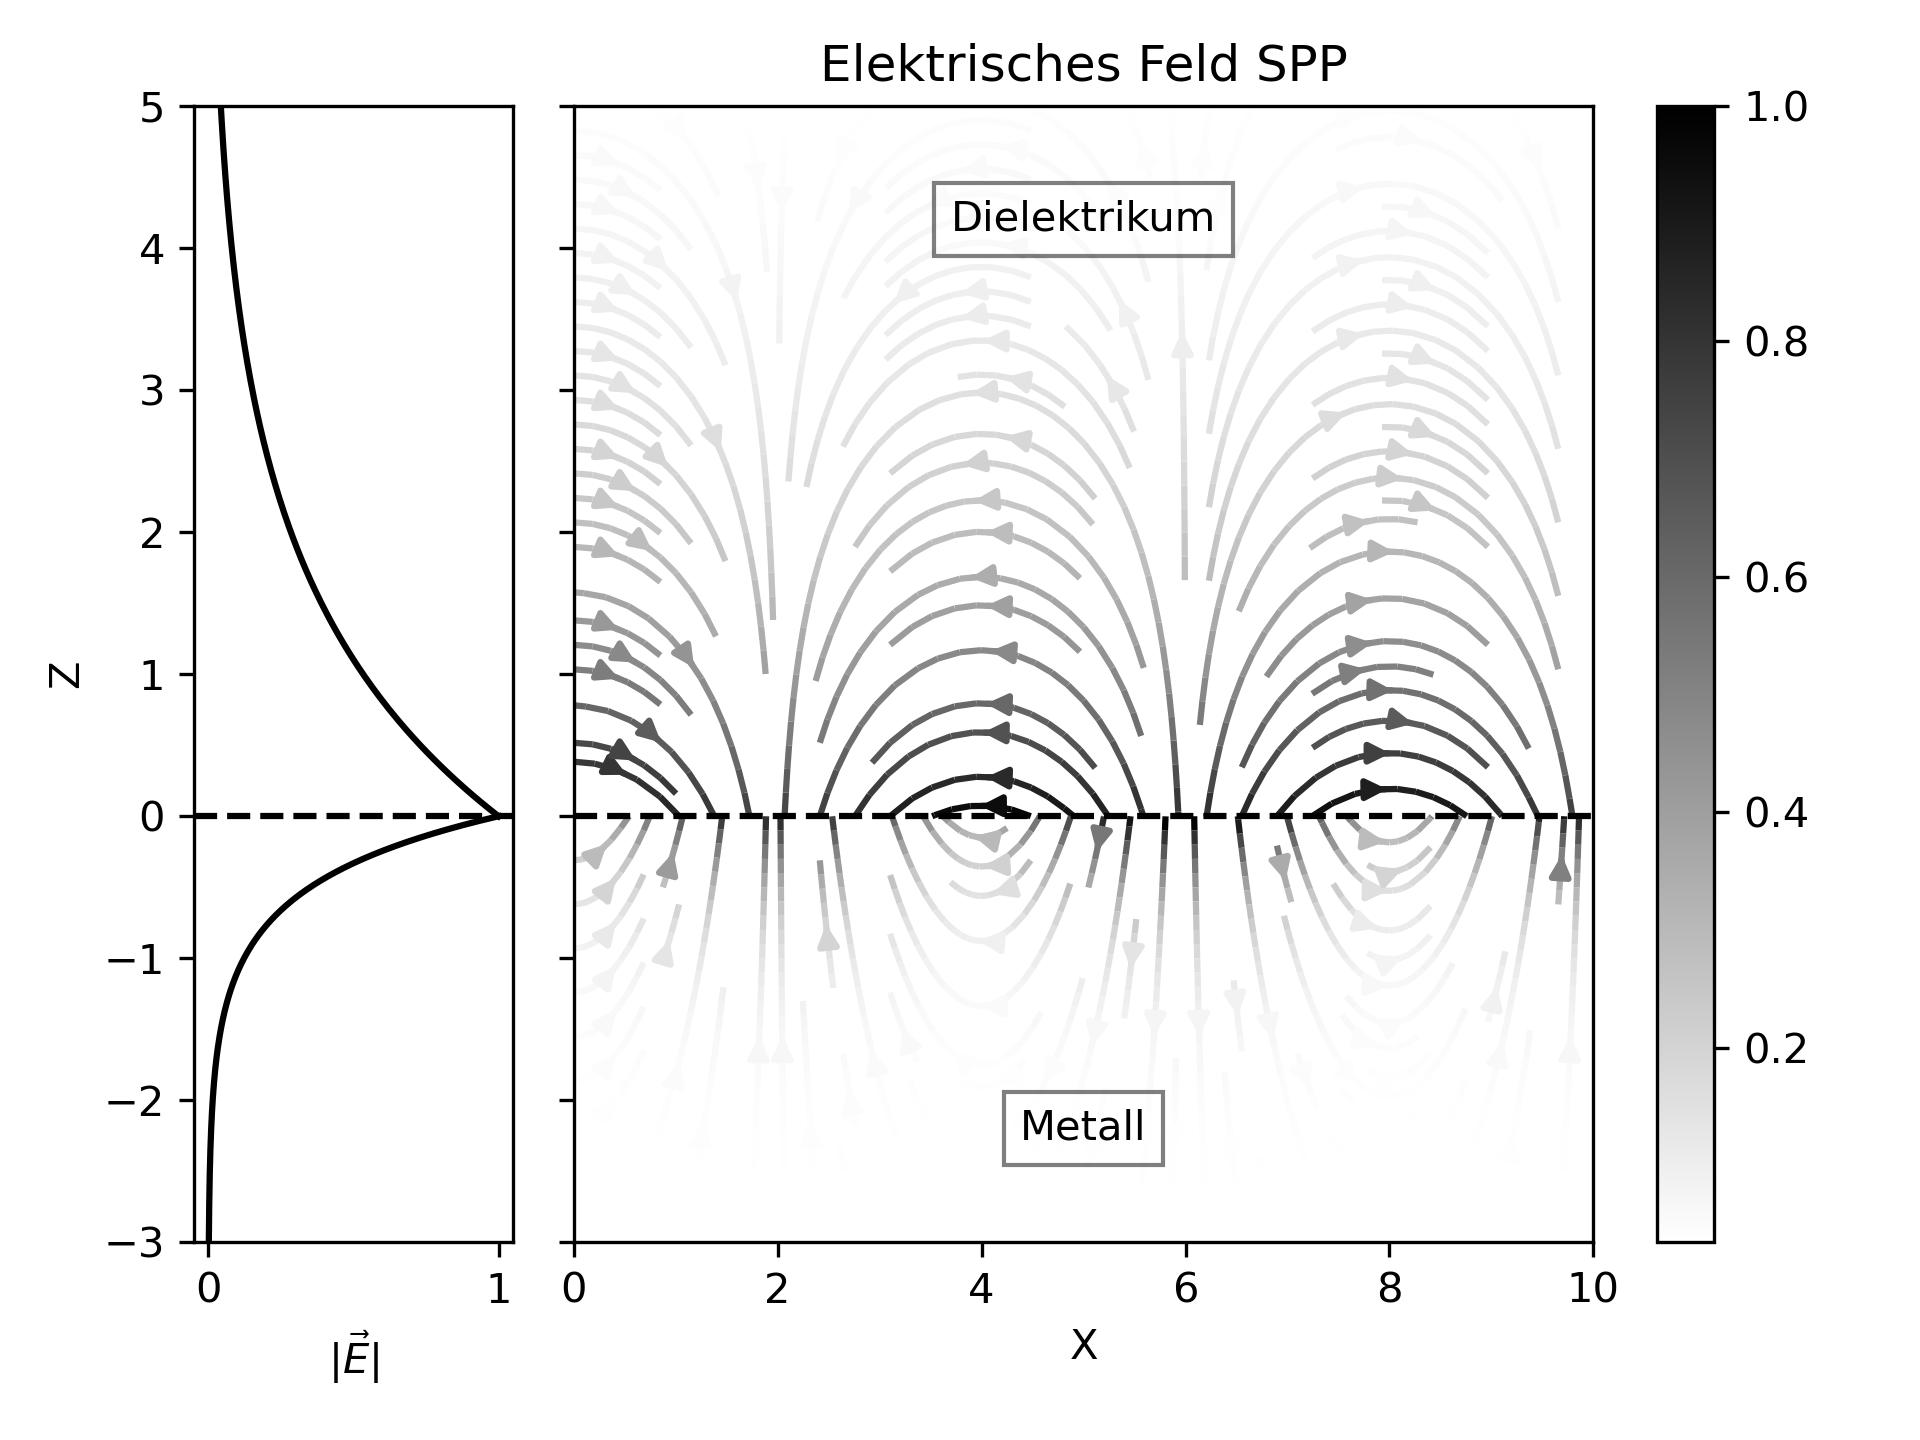
\includegraphics[width=0.7\textwidth]{figures/E_Feld_SPP.png}
		\caption{Elektrisches Feld eines SPP in der xz-Ebene mit $\vec{k}_{spp} \parallel \hat{e}_x$}
		\label{fig:electric_field_spp}
	\end{figure}
	Das Quant einer kollektiven Anregung eines Plasmas bezeichnet man als Plasmon. Ein Plasma hat unterschiedliche Anregungsmoden, die sich aus den Maxwellgleichungen und den Bewegungsgleichungen der geladenen Teilchen des Plasmas ergeben. Jede dieser Anregungsmoden wird durch spezifische Dispersionrelationen charakterisiert. Eine Dispersionrelation gibt an den Zusammenhang zwischen räumlicher und zeitlicher Verteilung der Wellenphase an.\cite{Fox.2020}\\
	
	Die einfachste Anregungsmode ist ein sogenanntes Volumenplasmon. Hierbei handelt es sich um eine Elektronendichtewelle. Durch die Bewegung eines Elektrons, vor dem positiven Ionen-Hintergrundes entsteht ein Netto-Elektrisches Feld, welches als Rücktreibende-Kraft auf das Elektron wirkt. Durch den rein longitudinalen Charakter dieser Rücktreibenden-Kraft ist auch die Elektronendichtewelle rein longitudinal. Daher ist es nicht möglich, ein Volumenplasmon mit Hilfe von elektromagnetischer Strahlung anzuregen, da Elektromagnetische Wellen im Vakuum rein transversal sind. Das heißt, dass sowohl das Elektrische, als auch das Magnetische Feld immer senkrecht auf der Ausbreitungsrichtung der Welle steht.\\
	
	Betrachtet man nun, statt einem unendlich ausgedehntem Plasma, die Grenzschicht zwischen einem Dielektrikum und einem Plasma, ergeben sich für diese aufgrund der besonderen Geometrie weitere Anregungsmoden. Eine davon ist das sogenannte Surface-Plasmon-Polariton (SPP). Hierbei handelt es sich um eine Anregung, die in ihrer räumlichen Ausdehnung eng an die Grenzschicht zwischen Plasma und Dielektrikum gebunden ist. Die elektrische und magnetische Feldstärke der Anregung fällt senkrecht zur Grenzschichtebene exponentiell ab. Man spricht von deshalb einem evaneszenten Feld. Das magnetische Feld dieser Mode ist rein Transversal. Das elektrische Feld weist im Gegensatz zu elektromagnetischer Strahlung im Vakuum sowohl transversale als auch longitudinale Komponenten auf. Durch den transversalen Charakter ist eine Kopplung zwischen SPP und elektromagnetischer Strahlung im Vakuum tendenziell möglich.

	\subsubsection{Dispersion}
	Aus den Maxwellgleichungen ohne externe Ladungen und Ströme \eqref{eq:maxwell} lässt sich mit Hilfe des Ansatzes $\vec{E}\left(\vec{r},t\right) = \vec{E}\left(\vec{r}\right) \exp\left(-i\omega t\right)$ die Helmholtz Beziehung \eqref{eq:helmholtz} herleiten.
	\begin{align}
		\label{eq:maxwell}	
		&\vec{\nabla}\cdot\vec{D} = 0		&\vec{\nabla}\cdot\vec{B} = 0 \\
		&\vec{\nabla}\times\vec{E} = -\dfrac{\partial\vec{B}}{\partial t} 
		&\vec{\nabla}\times\vec{H} = 	\dfrac{\partial\vec{D}}{\partial t}\nonumber
	\end{align}

	\begin{equation}
		\label{eq:helmholtz}
		\vec{\nabla}^2\vec{E} + k_0^2\epsilon_n\vec{E} = 0
	\end{equation}
	$k_0 = \dfrac{\omega}{c}$ ist hierbei die Wellenzahl einer elektromagnetischen Welle im Vakuum. Um nun aus der Helmholtz-Beziehung die explizite Dispersion eines SPP herzuleiten, ist es zunächst notwendig, die exakte Geometrie der Propagation zu definieren. Als Geometrie wählen wir zwei Halbräume, die durch die xy-Ebene von einander getrennt werden. Das SPP propagiert in dieser Ebene entlang der x-Achse. Außerdem gehen wir davon aus, dass die Anregung senkrecht zur Ausbreitungsrichtung in der xy-Ebene konstant ist. $\epsilon = \epsilon\left(z\right)$ sei ausschließlich eine Funktion von z. Das elektrische Feld der Anregung kann jetzt als $\vec{E}\left(x, y, z\right) = \vec{E}\left(z\right)\exp\left(ik_x x\right)$ geschrieben werden. $k_x = k_{spp}$ wird auch als Propagationskonstante der Anregung bezeichnet. Wenn man dieses elektrische Feld nun in die Helmholtz-Beziehung \eqref{eq:helmholtz} einsetzt ergibt sich die Wellengleichung:
	\begin{equation}
		\label{eq:spp_waveeq}
		\dfrac{\partial^2\vec{E}\left(z\right)}{\partial z^2}+ \left(k_0^2\epsilon-k_{spp}^2\right)\vec{E} = 0
	\end{equation}
	Aus dieser Wellengleichung lässt sich, wie detailliert in \cite{Maier.2007} gezeigt, die Dispersionsrelation einer Transversal-Magnetischen Mode (TM) berechnen:
	\begin{equation}
		\label{eq:dispersion_spp}
		k_{spp}\left(\omega\right) = \dfrac{\omega}{c} \sqrt{\dfrac{\epsilon_D\epsilon_M(\omega)}{\epsilon_D + \epsilon_M(\omega)}}
	\end{equation}
	Hierbei ist $\epsilon_D$ die Permittivität im Dielektrikum und $\epsilon_M(\omega)$ die im allgemeinen komplexe und frequenzabhängige Permittivität des Metalls.
	

	Aus den Maxwell-Gleichungen und den Randbedingungen an der Grenzschicht lässt sich wie in   die folgende Dispersionsrelation herleiten: $k(\omega) = ...$ Als Parameter wählen wir für das Plasma die Dielektrische Funktion von Gold und für das Dieelektrikum die Dieletrische Funktion von dem Glas des Substrates. Vergleicht man die so theoretisch berechnete Dispersion des SPP mit der Dispersion einer Elektromagnetischen Welle im Gold (ngold = ...), fällt auf, dass es zwischen den beiden Kurven keine Schnittpunkte gibt. Bei gleicher Anregungsfrequenz bzw. Energie haben die beiden Wellen unterschiedliche Räumlichefrequenzen. Dieser Missmatch in den Disipersionrelationen verhindert eine direkte Anregung, da zwischen Elektromagnetischer Welle und SPP beim ausbreiten auf der Probe eine zunehmende Phasendifferenz auftreten würde. Diese Problem kann durch unterschiedliche Mechanismen umgangen werden.		
		\subsubsection{Anregung}
			\paragraph{Kretschman-Konfiguration}
			\paragraph{Defekt-Anregung}
		\subsubsection{Leckstrahlung}
	\subsection{Plasmonischer-Spin-Hall-Effekt}
	\subsubsection{Spin SPP, Photon}
		\paragraph{Transversal-Spin SPP}
		\paragraph{Longitudinal-Spin Photon}
	\subsubsection{Nahfeld zirkular-polarisierter Dipol}
	\subsection{Gerichtete Anregung durch anisotropes Nahfeld}	
\section{Messung und Methoden}
\subsection{Polarimeter, Verzögerungsplatte, Lineare Dichroismus}
	\subsubsection{Dichroismus}
	\subsubsection{Doppelbrechung}
	\subsubsection{Jones-Formalismus}
\subsection{Leckstrahlmikroskopie}
	\subsubsection{Immersionsobjektiv}
	\subsubsection{Fourier-Optik}
\subsection{Optischer Aufbau}
\subsection{Probe}
\subsection{Justage und Kalibrierung}
\section{Ergebnisse und Diskussion}
	\subsection{Bestimmung des Polarisationszustandes}
		\subsubsection{Modellierung Jones-Polarimeter}
		\subsubsection{least-square-fit}
	\subsection{Bestimmung des Kontrastverhältnisses linkes/rechtes SPP}
	\subsection{Diskussion}
	\begin{figure}[htbp] 
		\centering
		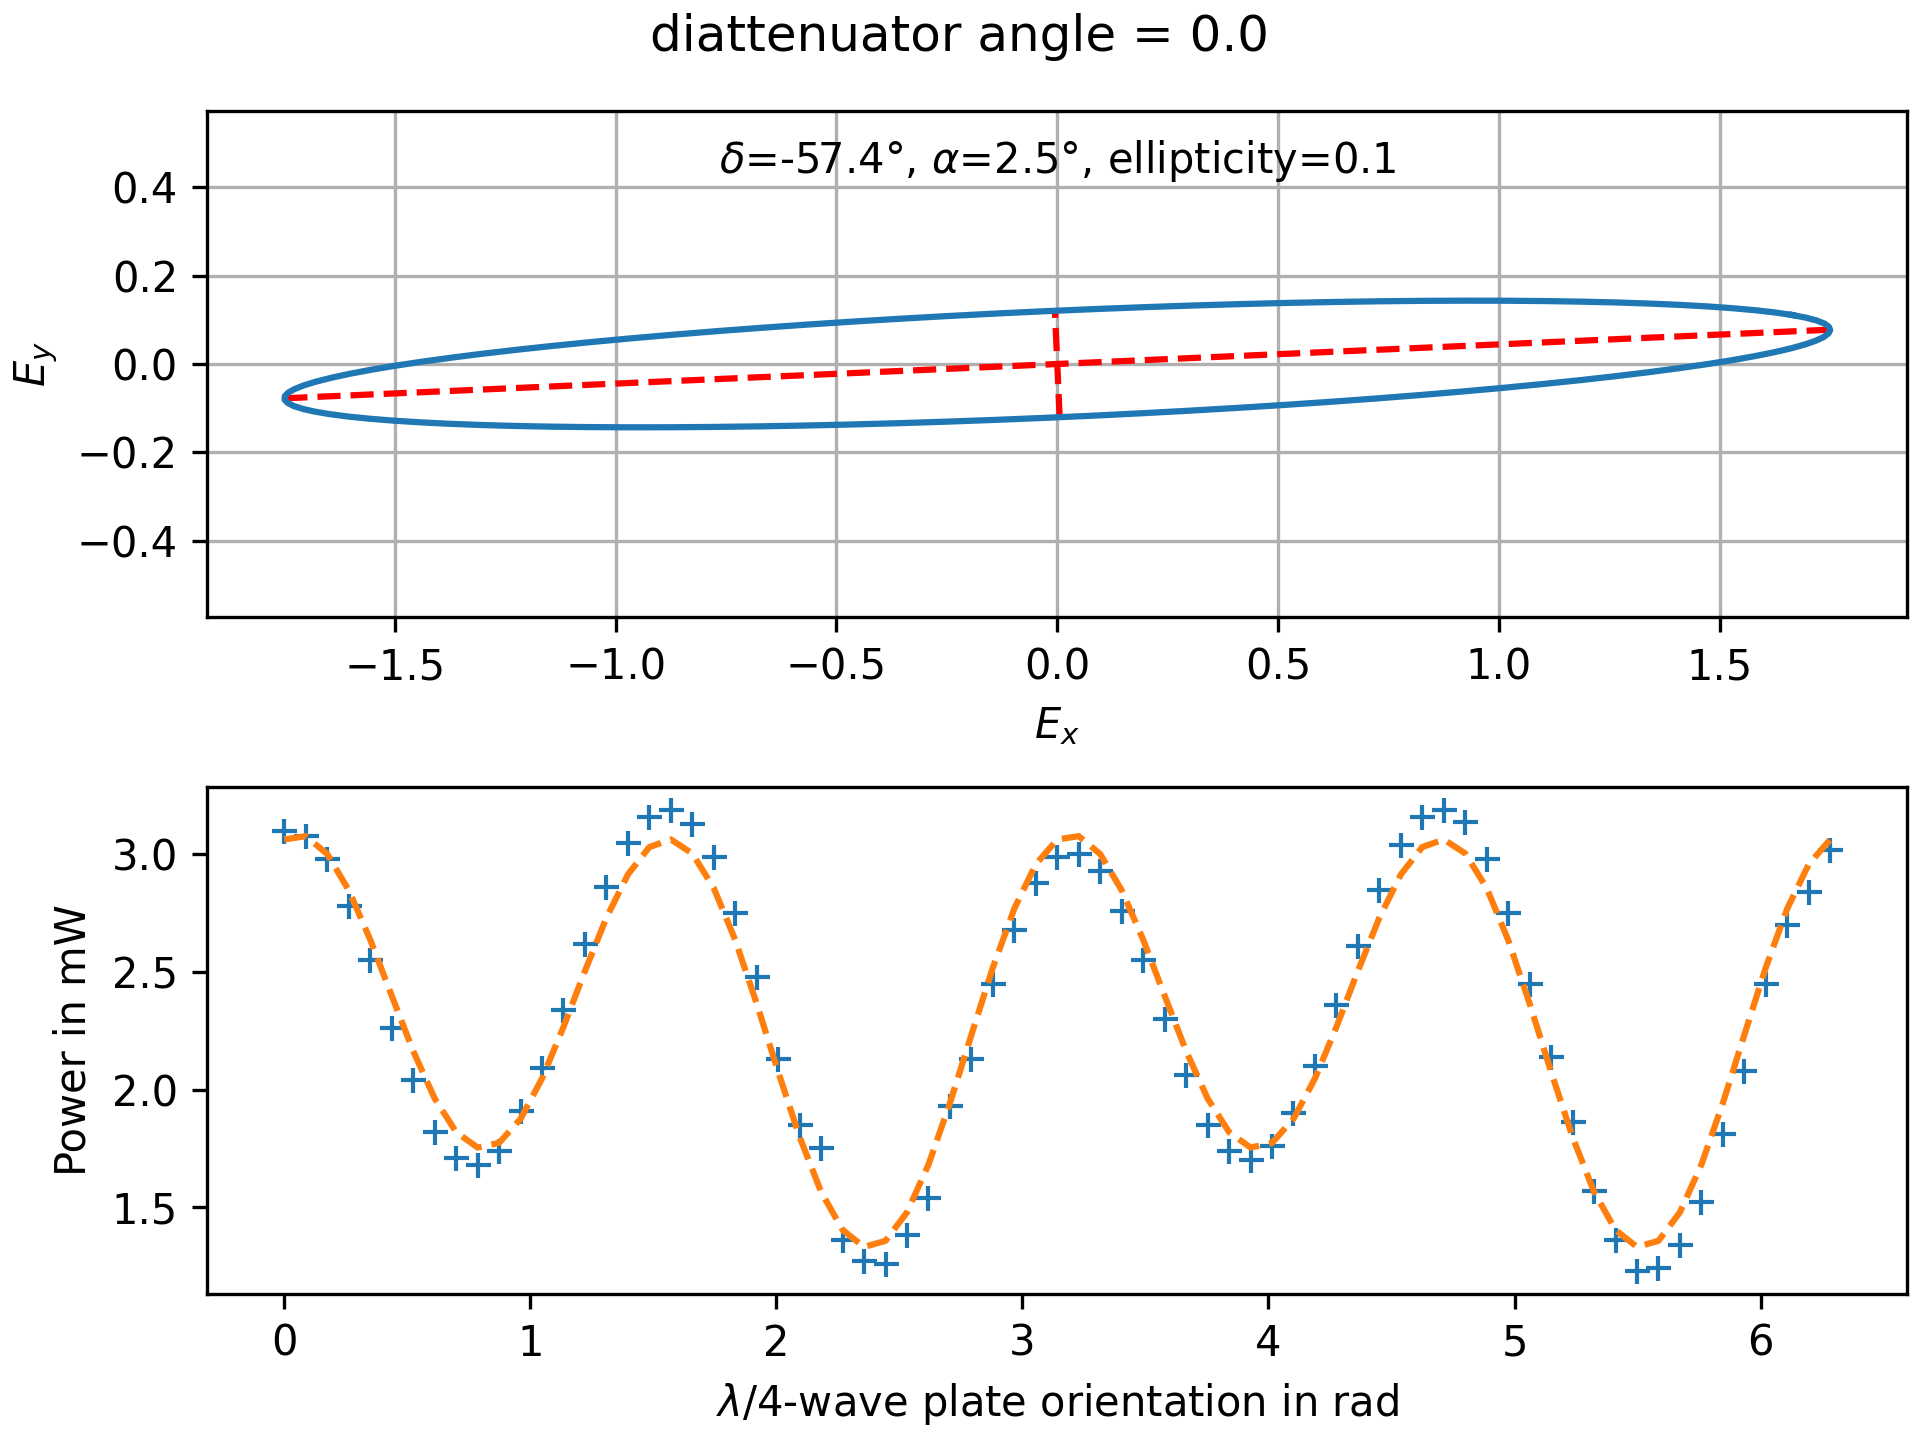
\includegraphics[width=0.7\textwidth]{figures/polarimeter.png}
		\caption{Polarisation}
		\label{fig:polarimeter}
	\end{figure}
\section{Zusammenfassung und Ausblick}
\newpage
\bibliography{bib}
	
\end{document}